
\chapter{Implementing object detection}
\label{objectDetection}
This chapter focuses on the process of detecting objects implemented by this thesis. The most basic knowledge was gained from Redmon's \cite{Redmon_2016_CVPR} article on YOLO architecture. Further, more general knowledge on the overall process and training was gained from the YouTube series and Ultralytics' documentation and tutorials \cite{objectDetectioProcessYT_general, objectDetectioProcessYT_ultralitics}.

The chapter starts by explaining why and how image data needs to be changed before being used by the object detection model. This is followed by an explanation of what the inference runtime is and which one is used in the thesis. Lastly, the chapter explains the steps taken during the extraction of detections from the outputs of the model. 

% ===========================================================================================

\section{Image preprocessing}
\label{imagePreprocessing}
Neural networks used for object detection are usually trained on preprocessed image data. Real world data are usually noisy, incomplete, inconsistent, and unbalanced. Preprocessing aims to clean these impurities and gives neural networks space to learn the important features needed for performing their tasks \cite{glossaryImagePreprocessing}. When passing image data into the neural networks, it is beneficial for the data to be preprocessed in the same way as it was during its training to achieve better results. 

\begin{figure}[hbt]
	\centering
	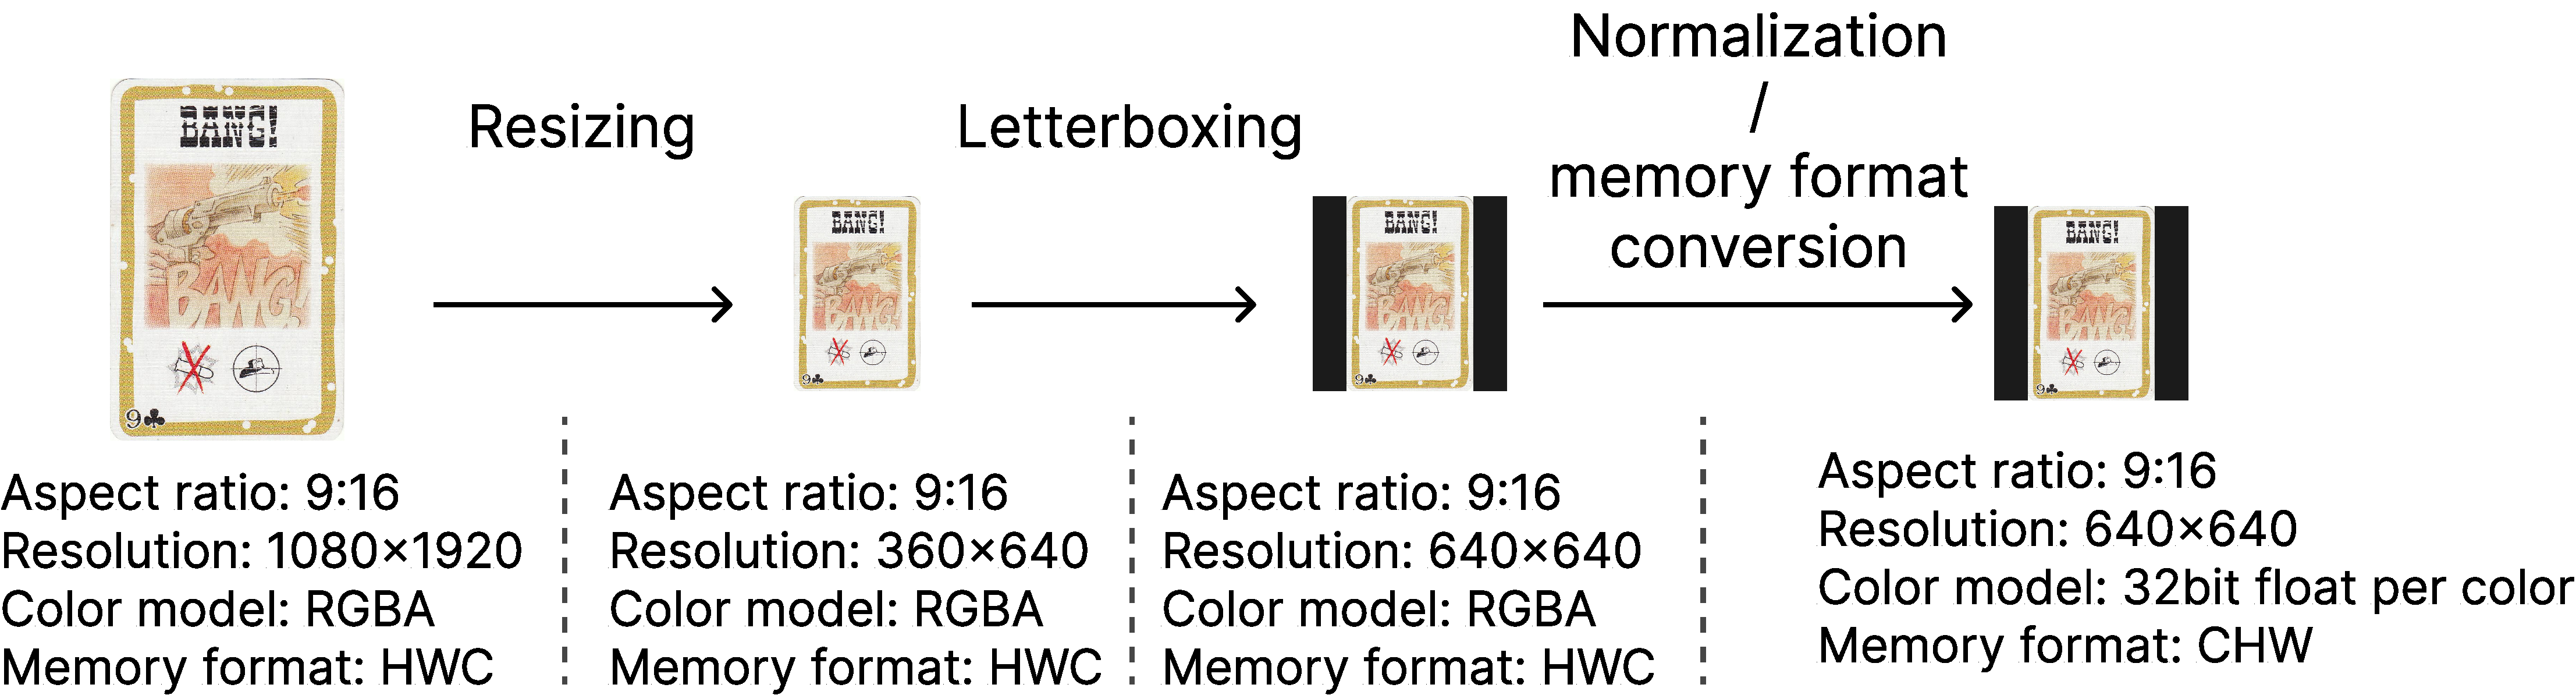
\includegraphics[width=1.0\textwidth]{obrazky-figures/preprocessing.pdf}
	\caption{Preprocessing steps shown on scan of the Bang! card from the game Bang!.}
	\label{preprocessingFigure}
\end{figure}

\subsection{Letter-boxing and resizing}
\label{letterboxing}
Some object detection models need a fixed resolution in order to perform object detection tasks. However, the image data provided by the camera might not always be in the correct resolution, therefore, rescaling is needed \cite{letterboxingAndNormalization}.

For example, using a camera that provides a resolution of \texttt{1080x1920} in portrait mode, and the model, which requires an image with a resolution of \texttt{640x640}. Rescaling the image would create a \texttt{640x640} image; however, the original aspect ratio of the image was \texttt{9:16}. This would change to a \texttt{1:1} aspect ratio, and the distortion could affect object detection.

Instead, both dimensions will be scaled by the same scale factor, using the larger dimension, resulting in an image with a \texttt{640x360} resolution. However, this results in only one of the dimensions not satisfying the resolution required by the model. \textbf{Letter-boxing} fixes this problem by padding the image with a value/color in one of the dimensions. This will result in a final image not being distorted and in the correct \texttt{640x640} resolution.


\subsection{Normalization and representing colors in a image}
Images can be represented as a matrix or a 2-dimensional array of pixels, where each pixel is represented by three values: red, green, and blue. Most image formats use 8 bit or 16 bit unsigned integers for each color channel. This format is known as 8 bit or 16 bit RGB format, respectively. However, neural networks are mostly trained on normalized float values. Each color channel is converted into a float and normalized by the maximum value of the format; for 8 bit, this is \texttt{255}.

\subsection{Converting colors channel formats}
The section above explained different ways of representing the values of each pixel in the image. However, the formats used to store these values in memory differ based on the needs of computer vision. Probably the most commonly used and intuitive way of storing image data is to use a 2-dimensional matrix of pixels, where each pixel is composed of three color values. This is called \textbf{HWC} format: Height x Width x Channel, where the channel refers to color values. For RGB format, there are three channels.

\begin{figure}[hbt]
	\centering
	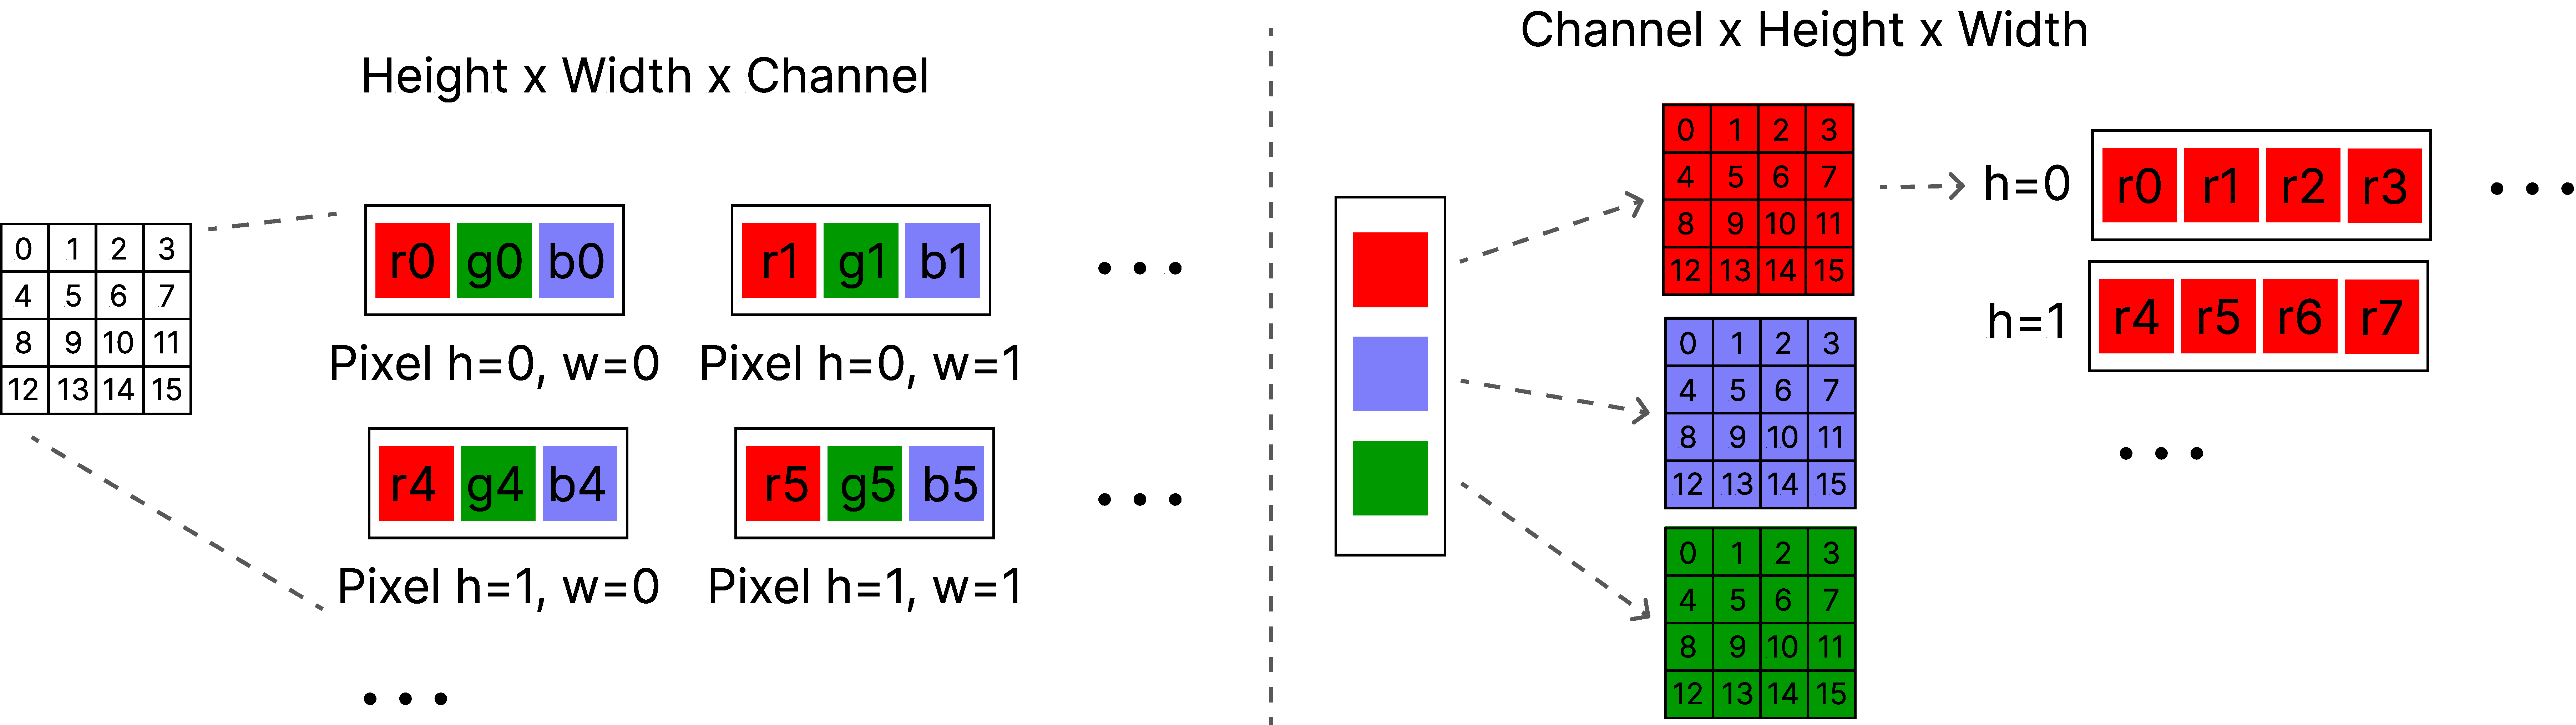
\includegraphics[width=1.0\textwidth]{obrazky-figures/channels.pdf}
	\caption[Image memory data layout of HWC and CHW]{Figure showing difference between HWC on the left, and CHW on the right. Both show 4x4 image with 3 color channels.}
	\label{ChannelsFigure}
\end{figure}

The commonly used format in neural networks, especially those aimed at image processing, is \textbf{CHW}. This format represents the image data in 3 sets of 2-dimensional matrices, each matrix containing values for a specific color, considering we are using RGB format with 3 color values \cite{channelFormatsSynopsis}. This format is beneficial for GPUs and NPUs as it is more suited for operations performed by these accelerators, especially parallel and vector operations \cite{chwAndHwcFormats}. 

A simple example of in-memory arrangement for these two formats for images with 3 color channels for a 2x2 image:

\begin{verbatim}
HWC
r0, g0, b0, r1, g1, b1, r2, g2, b2, r3, g3, b3

CHW
r0, r1, r2, r3, g0, g1, g2, g3, b0, b1, b2, b3
\end{verbatim}

Neural networks trained on data in \textbf{CHW} format will also expect this format during inference runs, meaning all image data used for object detection by the neural network must be converted to this format as well.


% ===========================================================================================

% ===========================================================================================

\section{Inference}
Inference in machine learning refers to the process of using a trained model to make predictions or decisions. This process applies the knowledge learned by the model and applies it onto new, unseen data, essentially solving real-world problems \cite{lenovoInference}. This task is performed by the \textbf{inference runtime}.

\subsection{Choosing an inference runtime}
\label{chosingInferenceRT}
To deploy a deep learning–based object detection model on embedded or mobile devices, a dedicated inference runtime is required. Inference runtimes or engines are responsible for executing trained neural network models by loading the model parameters, processing input data, and producing task-specific outputs. In this work, the runtime executes object detection using the deployed model to perform real-time object detection on image data.

OpenCV can be used as an inference runtime for CNN based neural networks with its \textit{Dnn} package. However, this approach was replaced after the first trial deployment due to insufficient performance, and further research was performed. 

More popular and widely used inference runtimes are TensorFlow Lite and Open Neural Network Exchange Runtime (hereinafter referred to as ONNX and ORT for the runtime). Both runtimes also support mobile devices. A study from 2023 \cite{Ren2023_ONNX_TensorFlow_BScan} shows ONNX out-performing TensorFlow on both CPU and GPU. The other blog post \cite{aimtechnoOnnxTFcomparison} from 2025 shows the gap closing as the performance difference between the runtimes is decreasing, with both having their pros and cons. The study also points out the open nature of the ORT and its more multi-platform development approach, whereas TensorFlow Lite can benefit from Google's ecosystem. The ONNX Runtime was chosen as the main inference runtime. However, since the CVLiBG was designed to be expandable and modular, adding another runtime should be an easy task for developers interested in different approaches.


% ===========================================================================================

% ===========================================================================================

\section{Postprocessing}
After preprocessing, the image was transformed into a suitable format usable by the neural network. The results of this inference run are further processed. This step is called \textbf{postprocessing}, and its purpose is to extract usually raw float values into more structured data, ultimately resulting in sets of detected objects. 

\subsection{Data extraction}
The first step is to extract the data from the output type of the inference engine into a more developer-friendly array style. Both \texttt{YoloOnnxDetector} and \texttt{YoloOpenCVDetector} have different types of outputs (these detectors are further discussed in \ref{Detector}). However, both of these \texttt{Detectors} outputs can be converted to a 1-dimensional array of float values.

In order to extract values, it is necessary to know the layout of the data, which for YOLO neural networks converted to ONNX format is: \texttt{[batch]x[attributes]x[detections]}. Where the \textbf{batch} is always 1 because \texttt{Detectors} work only with a single image; therefore, the shape is effectively \texttt{[attributes]x[detections]}. The \textbf{attributes} are individual values from the detection, meaning: x, y, width, height, and confidence score of each class. \textbf{Detections} refer to the number of detections found by the model. For the YOLOv8 models, this value represents grid like feature maps: 80x80 + 40x40 + 20x20 = 8400 \footnote{How YOLOv8 Works: \url{https://nvidia-isaac-ros.github.io/concepts/object_detection/yolov8/index.html\#how-yolov8-works}}.

\begin{figure}[hbt]
	\centering
	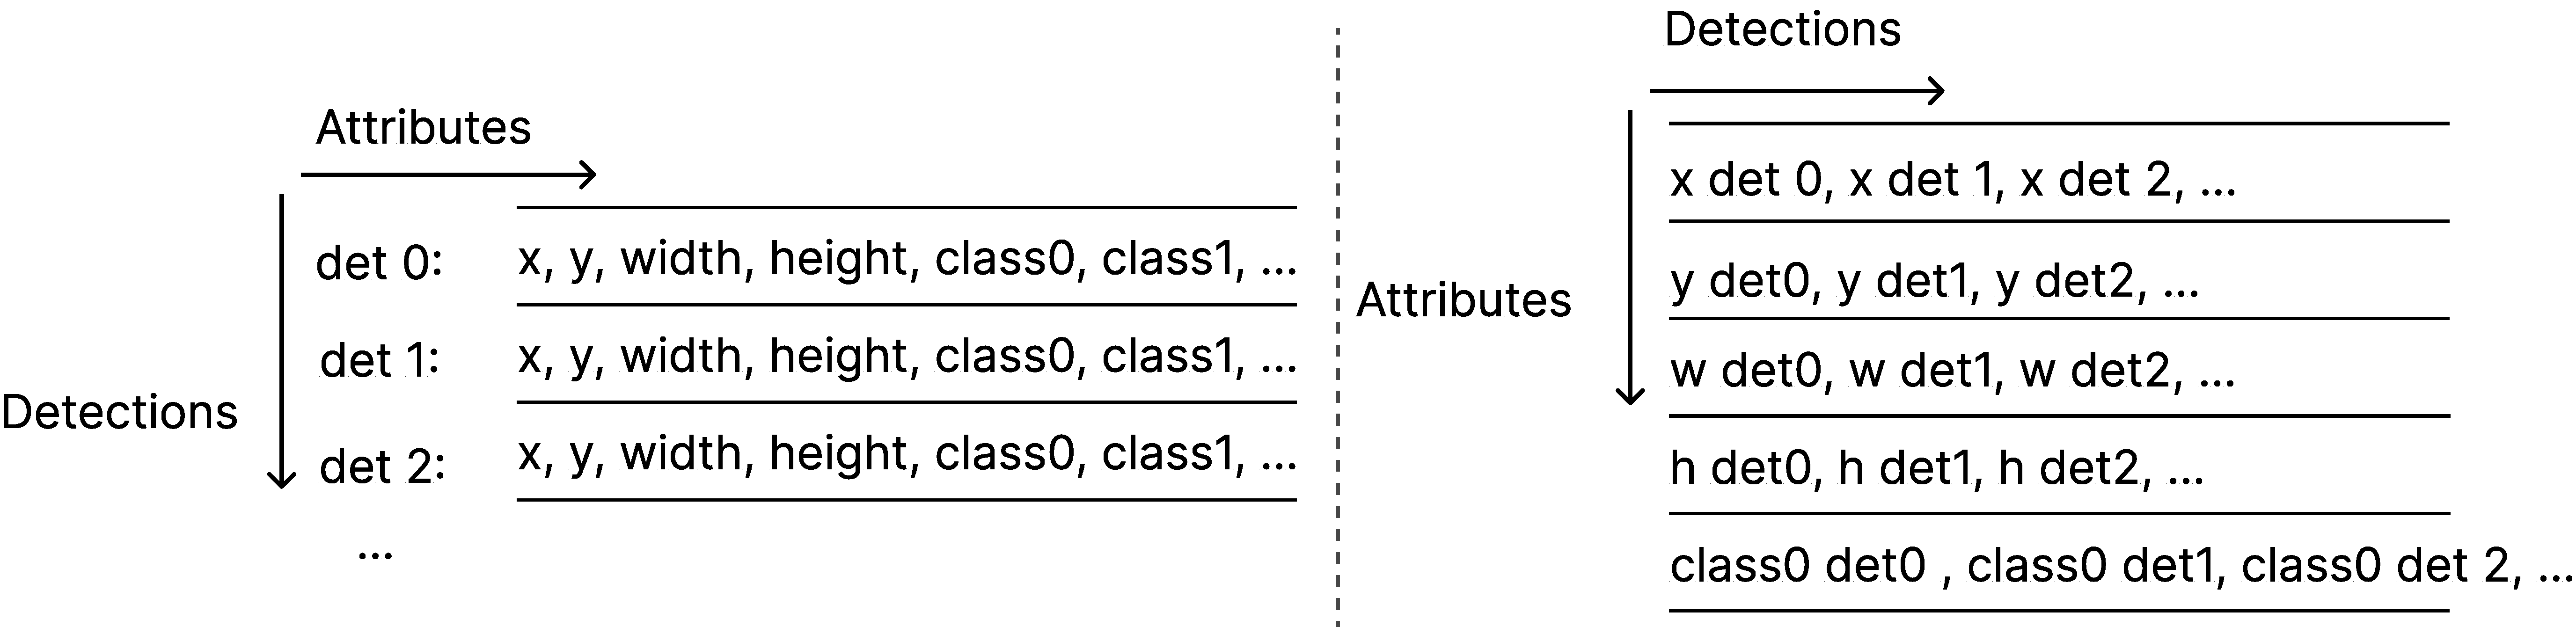
\includegraphics[width=0.98\textwidth]{obrazky-figures/extracted_data_layout.pdf}
	\caption[Memory layout of raw extracted detections]{Figure showing data layout in memory, on the left [detections]x[attributes], on the right [attributes]x[detections].}
	\label{ExtractedDataLayoutFigure}
\end{figure}

However, the \texttt{[attributes]x[detections]} shape might not be the most intuitive one. Therefore, there are two options: use it as it is or transpose the data. Both are valid options, and in mathematics, transposing might be preferred. However, performing these operations on already resource limited devices is not an optimal solution.

\begin{verbatim}
// data : array containing data in [attributes]x[detections] format 
for (column in 0 until numberOfDetections) {
    val x = data[0 * numberOfDetection + column]
    val y = data[1 * numberOfDetection + column]
    // ...
}    
\end{verbatim}

\begin{verbatim}
// data : array containing data in [detections]x[attributes] format 
for (attributes in data) {
    val x = attributes[0]
    val y = attributes[1]
    // ...
}    
\end{verbatim}

The abstract code snippet above shows the difference between the two approaches. A very simple test for both of these methods shows that transposing the data is 3 times slower, which is approximately \texttt{5.18 milliseconds}. Therefore, a direct approach mirroring the memory layout was chosen as the final solution for both included \texttt{Detectors}.

\subsection{Thresholding}
The result of the extraction step is a list of \texttt{Detection} (see \ref{DetectionClass}) objects. Each object contains x and y coordinates, height and width dimensions, and its best class and confidence score. However, before creating an object, all confidence scores for the given detection are compared, and the highest value and its class are stored. If the best confidence score value is above the \textbf{threshold}, an object will be created; otherwise, this detection will be filtered out.

\begin{verbatim}
var bestClass : Int = -1
var bestScore : Float = 0f

for (row in 4 until numOfAttributes) {
    val score = data[row * numOfDetections + column]
    if (score > bestScore) {
        bestClass = row - 4
        bestScore = score
    }
}
\end{verbatim}

Lastly, it is necessary to determine the best class with the highest confidence score. This is done by retrieving all confidence scores and simply remembering the highest value and the index.


\subsection{Non-Maximum Suppression}
The object detection model might output multiple bounding boxes for one object. These duplications need to be removed, and the most proven method is \textbf{Non-Maximum Suppression} \cite{nms}. If the computed \textbf{Intersection Over Union} or \textbf{IoU} for two detections is past a threshold, the detection with the lower confidence score is removed. The NMS algorithm can be simplified into 3 steps \cite{nms}:

\begin{enumerate}
  \item {Choose the detection with the highest confidence score from all detections, remove it from the list of all detections, and add it to the list of kept ones.}
  
  \item {Compute IoU for the chosen detection, from the 1st step, and the rest of the detections. If the IoU is above the threshold, remove it from the list of all detections.}
  
  \item {Repeat until the list of all detections is empty.}
\end{enumerate}

\begin{verbatim}
allDetections.sortByDescending { it.score }
keptDetections = mutableListOf<Detection>()
while (allDetections.isNotEmpty()) {
    val best = allDetections.first()
    keptDetections.add(best)
    allDetections.remove(best)

    for (detection in allDetections) {
        if (computeIoU(best, detection) > threshold)
            allDetections.remove(detection)
    }
}
\end{verbatim}

The code above shows the implementation of NMS. The list of detections is sorted by confidence score at the start instead of looking for the best score in each step. It should be noted that this code does not work and is not used, as deleting an item from the list while iterating through it will result in an error. Instead, a method with boolean masks is applied. This method masks detections instead of removing them; these can be skipped without the need for deleting objects from the list. However, this version was chosen for illustration purposes as it is more straightforward .

\begin{figure}[hbt]
	\centering
	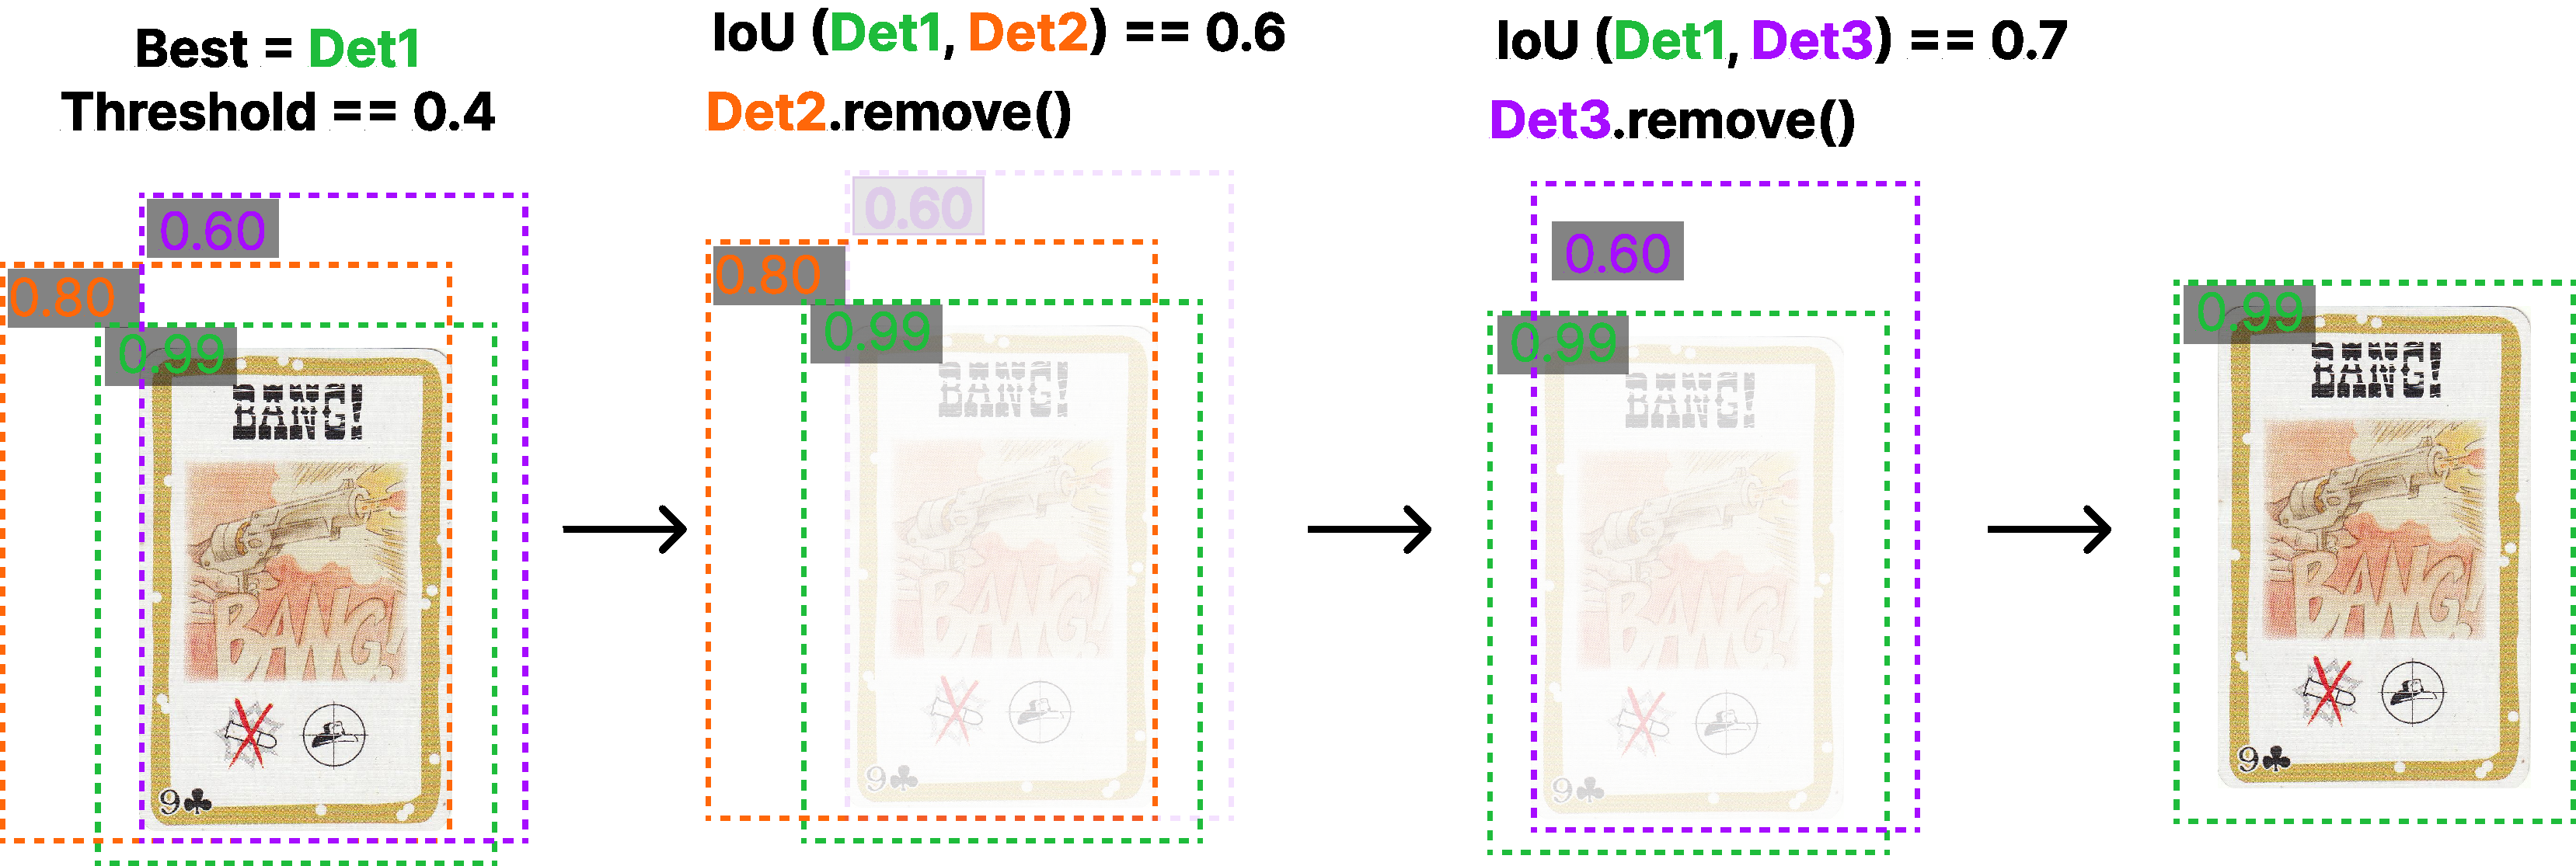
\includegraphics[width=0.80\textwidth]{obrazky-figures/nms_example.pdf}
	\caption{Simplified Non-Maximum Suppression demonstration.}
	\label{nsmDemonstration}
\end{figure}

This, however, can result in objects of different classes removing one another. For example, an apple held by a person is being deleted because it overlaps with a human who has a higher confidence score. To help solve this problem, NMS is applied only to the same classes; therefore, only the human class can remove another human class.

CVLiBG also contains another implementation of NMS using OpenCV's built in NMS filtering method. However, this method requires converting the \texttt{Detection} objects into OpenCV's \texttt{Rect2D} objects. This method is \texttt{1.5} to \texttt{2} times slower, with a time difference of 63 nanoseconds, compared to the method written in Kotlin using \texttt{Detection} objects.

NMS is not a cheap operation, especially with many objects in one scene, as it has to iterate through all detected objects multiple times. Therefore, it is recommended to first reduce the number of detections using thresholding or other methods \cite{nms}. Lastly, NMS can use confidence softening instead of removing detections. However, this approach was implemented for real-time detection tasks as it would require multiple repetitions. 

\bigskip
\textit{Note: all of the above mentioned data showing performance comparisons between different methods were collected using the YOLOv8 model and on an available device whose hardware capabilities are mentioned in \ref{bangTrainingExperiments}.}